% !TEX encoding = UTF-8 Unicode
% !TEX root = project.tex

\section{Software Setup}
\label{sec:setup}

\begin{figure*}[ht!]
\centering
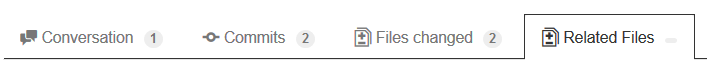
\includegraphics[width=16cm]{NewTabRelatedFiles}
\caption{GitHub pull request page showing the new `Related files' tab}
\label{fig:newTabRelated}
\end{figure*}

\begin{figure*}[ht!]
\centering
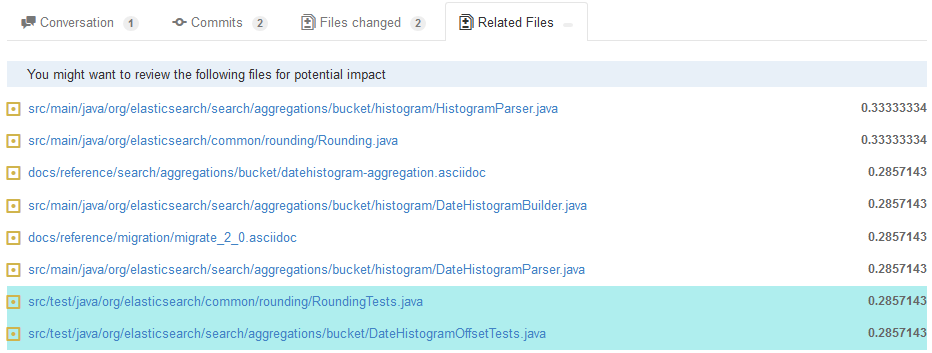
\includegraphics[width=16cm]{RelatedFilesContents}
\caption{`Related files' tab showing files}
\label{fig:relatedFilesContents}
\end{figure*}

\begin{figure*}[ht!]
\centering
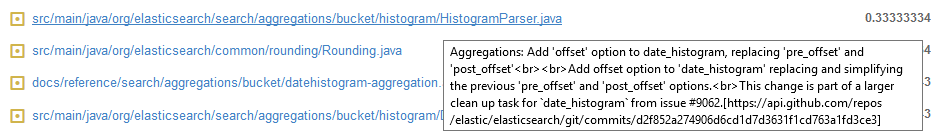
\includegraphics[width=16cm]{MouseOverOfFile}
\caption{Details of the file on performing mouse-over on the hyperlink}
\label{fig:mouseOverOnFile}
\end{figure*}

\begin{figure*}[ht!]
\centering
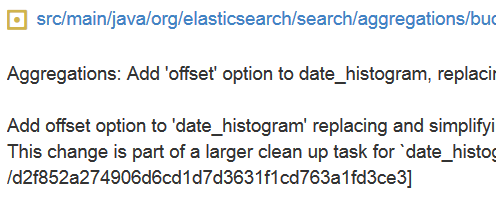
\includegraphics[width=16cm]{ClickOfFileHyperlink}
\caption{Details of the file on clicking on the hyperlink}
\label{fig:clickOnFileHyperlink}
\end{figure*}

The software setup was done on a single laptop having an Intel dual-core i5-4210U CPU running at 1.7 GHz with 8 GB RAM, with Windows 8.1 64 bit operating system. In our setup, we created a Javascript user script which was installed on the Firefox browser using GreaseMonkey add-on~\cite{greasemonkey1,greasemonkey2}. When this script is invoked on a Github pull request page, it adds a new tab named `Related Files' onto the page. Figure~\ref{fig:newTabRelated} shows a screenshot of the webpage showing the new tab. The tab, on opening, sends a REST~\cite{rest} POST~\cite{post_http} request with the all the files from the pull request in its HTTP message body. The REST service, which is deployed on a Glassfish server~\cite{glassfish}, receives the files send from the Github page. The REST service then makes use of the Top-K association rule mining algorithm~\cite{fournier2012mining} to come up with a list of related files and is send back to the Github page, i.e., from where the request was initiated. The Github page will display the results in the 'Related Files' tab. Test files are highlighted in a different color. 

Figure~\ref{fig:relatedFilesContents} shows the contents of the related files tab populated from the REST service output. A confidence value is shown against each file which is obtained from the association rule mining algorithm.

Figure~\ref{fig:mouseOverOnFile} shows what happens when the mouse is hovered over the hyperlink. It shows the reason why the particular file shows up on the related files tab.

Figure~\ref{fig:clickOnFileHyperlink} shows what happens when the hyperlink is clicked. It is the same reason as above, but user can copy the contents if required.

